\documentclass{article}
% HAIC @ NeurIPS 2026 is double-blind and non-archival.
\usepackage[dblblindworkshop, final]{neurips_2026}
\workshoptitle{Human-AI Coevolution: Measuring Human-Agent Teams in the Agentic Era}
\usepackage[utf8]{inputenc}
\usepackage[T1]{fontenc}
\usepackage[hidelinks]{hyperref}
\usepackage{url}
\usepackage{booktabs}
\usepackage{amsmath}
\usepackage{graphicx}
\usepackage{xcolor}

\title{Whose Gold? Annotator-Pool Disagreement Is Large at the Item Level\\and Invisible in a Six-Model Leaderboard}

\author{Anik Jha\\Independent Researcher\\\texttt{anik.k.jha@gmail.com}}


\begin{document}
\maketitle

\begin{abstract}
Preference benchmarks are built by hiring annotators, and the identity of those
annotators is treated as an implementation detail. We measure what that detail buys, on
two corpora that put \emph{predefined} annotator populations on the \emph{same} items.
On the $2{,}885$ \textsc{MultiPref} items where both pools are internally unanimous, so no
tie-breaking convention is consulted at all, the normal and expert-designated pools assign
a different majority label to $23.6\%$ and name the \emph{opposite winner} on $9.2\%$; on
the $246$ comparably unanimous \textsc{MT-Bench} cells, benchmark authors and recruited
experts differ on $30.5\%$ and reverse on $8.5\%$. Yet on both corpora the resulting
six-model \emph{orderings} are identical: Kendall $\tau = 1.00$, zero models displaced,
even though the win-rate vectors are not.

That invariance is weaker evidence than it looks, and the weakness is measurable on this
corpus rather than extrapolated. An item-level bootstrap of the real corpus displaces at least
one model in $27.9\%$ of resamples on the full corpus and $34.7\%$ on the convention-free
subset the headline uses, almost all of it at the one adjacent pair sitting $0.8$pp apart,
which the two golds order differently in $22.6\%$ of resamples. These are resampling
frequencies on this corpus, not a general probability of leaderboard change. The
observed zero is the modal outcome rather than a reliable one, not a property of
aggregation, and it is a statement about this leaderboard's spacing rather than about
leaderboards. The per-item consumer we test, three local LLM judges, leans toward the
normal pool by $1.8$--$3.5$pp after reweighting to the corpus when scored against
tie-broken pool majorities, with one of the three distinguishable from zero. That sign
depends on the tie-break: one judge reverses under the leaderboard's own rule, and a
per-annotator score that needs none leaves one judge with a lean distinguishable from zero.
We separate the two regimes. Within \textsc{MultiPref}'s expert-designated pool the two
annotators give different coarse labels on $50.1\%$ of comparisons, evidence against the
zero intra-group variability its routing model assumes and distinct from the between-pool
contrast its authors left for future work. Code, results and per-call judge outputs:
\url{https://github.com/anik-jha/whose-gold}.
\end{abstract}

\section{Introduction}

Every preference benchmark rests on a hiring decision. Someone chose whether to
recruit crowdworkers or domain experts, how many to put on each item, and how to
collapse them into a label. That choice is normally reported in an appendix and
then never mentioned again, because the field's implicit model is that annotators
are noisy instruments measuring a single underlying quantity.

The dataset we study states this assumption explicitly, for its routing model. \textsc{MultiPref}
\citep{miranda2024hybrid} deliberately collects two annotator pools and its Limitations
section says: \emph{``One of our key assumptions is that there is no variability in
intra-group annotators \ldots{} the dataset disambiguates between normal and expert
crowdworker annotations. We leave this exploration for future work.''} Both pools are
Prolific crowdworkers who passed the same qualification test; \textsc{MultiPref} designates
one of them \emph{expert} on education, a graduate degree where the other pool needed a
bachelor's, with prompts routed by academic domain, and we use its own labels for the two groups throughout rather than the
stronger word ``domain expert''. We therefore do not read the gaps below as a
crowd-versus-domain-expert gap.

Part of that exploration has been done. \citet{zhang2025diverging} study disagreement in
\textsc{MultiPref} and \textsc{HelpSteer2} directly, build a taxonomy of its causes, show
that most disagreement is not annotation error, and release
\textsc{MultiPref}-Disagreements. Their unit of analysis is the \emph{annotator pair}: they
take all permutations of \textsc{MultiPref}'s four annotators per item, which marginalises
over precisely the variable \textsc{MultiPref}'s own future-work note names. We condition on
it instead. That is the difference this paper turns on, and it buys two things Zhang et al.
do not report: a like-for-like contrast between two \emph{predefined populations} rating
identical items, and what that contrast does downstream to a model ranking and to an LLM
judge. Neither corpus-level disagreement nor its causes is our claim; the comparison
conditioned on a predefined pool is. Neither corpus assigns annotators to pools at random,
so the comparison is observational: it describes how two recruited populations label the
same items, not the effect of hiring one instead of the other.

A human-agent team is scored against exactly these labels. When a team's output is
graded, or a monitor is validated against ``human agreement'', the gold standard is
whichever pool was hired; if that choice moves half the item-level decisions, it
moves the measured competence of the team as much as the team does. That is the
sense in which this is a question about human-AI coevolution rather than about
dataset hygiene.

Our contribution is a measurement and a distinction:

\begin{enumerate}\itemsep2pt
\item \textbf{Item-level divergence between predefined pools is large.} Two pools
annotating the same items reverse the winner on $9.2\%$ (\textsc{MultiPref}, on the
$2{,}885$ items needing no tie-breaking convention) and $8.5\%$ (\textsc{MT-Bench},
likewise), and change the majority label on $23.6\%$ and $30.5\%$. On \textsc{MultiPref}
the two expert-designated annotators on a single item disagree with each other on the coarse
A/Tie/B scale $50.1\%$ of the time.
\item \textbf{None of it reaches \emph{this} leaderboard, and that is a statement about
spacing.} Ranking the same models under expert-gold and normal-gold labels gives
$\tau = 1.00$ on both corpora, with no model displaced. But an item-level bootstrap of the
same corpus displaces a model in $28\%$ of resamples, so the observed zero held here but
fails in more than a quarter of them, not a demonstration that aggregation absorbs the pool.
The $28\%$ describes this corpus under this resampling, not a general probability of
leaderboard instability (\S\ref{sec:threshold}).
\item \textbf{The distinction that follows.} These two six-model leaderboards keep their
ordering despite the item-level divergence; reward-model training, active-annotation
routing, and LLM-judge validation all consume \emph{per-item} labels and get no such
averaging. We measure one of these and \emph{conjecture} the others: only the judge is
tested here.
\item \textbf{One such consumer, measured, and how its measurement depends on aggregation.}
Three LLM judges, two from one vendor and one from another, all lean toward the normal
pool when scored against tie-broken pool majorities. Reweighted from our stratified sample
back to the corpus the lean is $-2.2$, $-3.5$ and $-1.8$pp, and one of the three has an
agreement CI excluding zero; on the sample as drawn all three are larger. That shared sign
depends on the tie-break (\S\ref{sec:judge}). ``Our judge agrees with humans $X\%$ of the time'' is therefore partly a
statement about the hiring decision and partly about how split pools were collapsed.
\end{enumerate}

\begin{table}[t]
\centering
\small
\caption{Headline numbers and the evidence behind each. \emph{Bootstrap}: frequencies under
prompt resampling of this corpus. \emph{Primary}: designated after the pre-registered sweep.
\emph{Exploratory}: added after review. $^{*}$: 95\% interval excludes zero.}
\label{tab:summary}
\setlength{\tabcolsep}{4pt}
\footnotesize
\begin{tabular}{llll}
\toprule
Finding & Number & Evidence & Where \\
\midrule
Label changes / reversals & $23.6\%$ / $9.2\%$ \textsc{MultiPref}; $30.5\%$ / $8.5\%$ \textsc{MT-Bench} & Measured & Table~\ref{tab:main} \\
Model ordering, both boards & $\tau = 1.00$, $0/6$ displaced & Measured & \S3 \\
Displacement under resampling & $27.9\%$ of resamples; $22.6\%$ at the $0.8$pp pair & Bootstrap & \S\ref{sec:threshold} \\
Boards with $K > 6$ models & not measured & Illustration & Table~\ref{tab:threshold} \\
Judge lean, original tie-break & $-2.2$, $-3.5^{*}$, $-1.8$pp & Primary & Table~\ref{tab:judge} \\
Judge lean, per annotator & $-1.6$, $-2.5^{*}$, $-0.6$pp & Exploratory & Table~\ref{tab:convention} \\
\bottomrule
\end{tabular}
\end{table}

\section{Setup}

\textbf{Corpora.} \textsc{MultiPref} \citep{miranda2024hybrid} contains $10{,}461$
pairwise comparisons over six models, each annotated twice by its \emph{normal} pool and
twice by its \emph{expert-designated} pool on a five-point preference scale. Both pools are
Prolific crowdworkers; the designation rests on education, not on a test of domain
competence, and we carry \textsc{MultiPref}'s own two labels rather than asserting a
stronger contrast than the dataset supports. \textsc{MT-Bench}
human judgments \citep{zheng2023judging} contains $3{,}355$ human votes; $292$
item cells are rated by both the benchmark's own authors (\texttt{author\_*}) and
recruited expert annotators (\texttt{expert\_*}), giving an independent pool
contrast over a different task and a different six-model set. The two contrasts differ in
kind, so agreement between them supports sensitivity to annotator source rather than a
shared expert-versus-normal mechanism.

We attempted two further corpora and report the failures, because they explain why this
contrast in particular went unmeasured. Both retain far more annotator information than we
need; what neither supplies is two \emph{predefined populations} rating the same items.
\textsc{PRISM} \citep{kirk2024prism} keeps participant identity and detailed
sociodemographic profiles, and studies how feedback varies across participants, but assigns
one participant per conversation; different participants rate an identical prompt-response
pair only where one happens to recur \citep[App.~S.5]{kirk2024prism}, so there is no
systematic fixed-item pool contrast. \textsc{HelpSteer2} keeps several annotators' ratings
per response, from which \citet{zhang2025diverging} derive preferences, and
\textsc{HelpSteer2-Preference} adds pairwise preferences from three to five annotators per
item \citep{wang2024helpsteer2, wang2024helpsteer2pref}, but their annotators come from one
vendor's pool with no predefined population split to condition on. The
scarce ingredient is not per-annotator labels; it is a pre-assigned population label
attached to them.

\textbf{Aggregation.} For each pool we take the majority label per item and score
a model by its mean credit over the comparisons it appears in. When a pool is split we resolve it by the
rule reported in the first row of Table~\ref{tab:tiebreak}, A over B over Tie, but the
primary analysis avoids the question entirely (see below). The judge arm of
\S\ref{sec:judge} used a different rule, A over Tie over B, for its sampling strata and its
reference labels. Rank comparisons use Kendall $\tau$ with a
\emph{paired cluster} bootstrap: each resample draws the same independent units for both
label sources, prompts for \textsc{MultiPref} and questions for \textsc{MT-Bench}, keeping
every comparison row of a unit together, since the two rankings differ only in whose labels
are used and both corpora reuse an item across model pairs.

\textbf{Pre-registration.} Decision rules were kept in a versioned plan; what preceded each
run is author-attested, not third-party registered. The plan's first committed version,
which predates the leaderboard results, held a $\tau$-only rule from an earlier team-level
design: if $\tau > 0.9$, report the null and do not enlarge the sweep. The conjunctive
form adding a CI lower bound $> 0.9$ first appears in the commit reporting the result, so
its timing is unverifiable. The observed $\tau$ meets the first rule but, given its wide
interval, not the conjunction; either way we report the null and did not enlarge the model
set.

\paragraph{Tie-breaking is not a detail here, so we avoid it.}
Each pool has two annotators and the two experts on an item give different coarse labels
on $50.1\%$ of items, so a ``pool majority'' is decided by convention on roughly half the corpus, and
the corpus is skewed $1.78{:}1$ toward B. Our primary analysis therefore consults no
convention: we restrict to the $2{,}885$ items ($27.6\%$) where \emph{both} pools are
internally unanimous. That conditions on the items both pools found easy, so $9.2\%$ is
not an unbiased estimate of the corpus reversal rate and it is not a bound on it in either
direction: across the five conventions of Table~\ref{tab:tiebreak} the rate runs from
$2.5\%$ to $29.8\%$, straddling it. What $9.2\%$ is, and what no other row in that table
is, is a number no tie-breaking rule of ours had a hand in.
Table~\ref{tab:tiebreak} gives the sensitivity. Our leaderboard ran a rule ranking A
over B over Tie. Four of five conventions, including the one we ran, leave the
ranking at $\tau = 1.0000$: under our own rule, $29.8\%$ of
items reverse and the leaderboard still does not move. One rule (A over Tie over B),
which our leaderboard did not use but our judge arm did, does break it ($\tau = 0.467$);
its mirror does not, so the ordering result depends on the aggregation convention.

\section{Divergence at the item level, invariance in aggregate}

\begin{figure}[t]
\centering
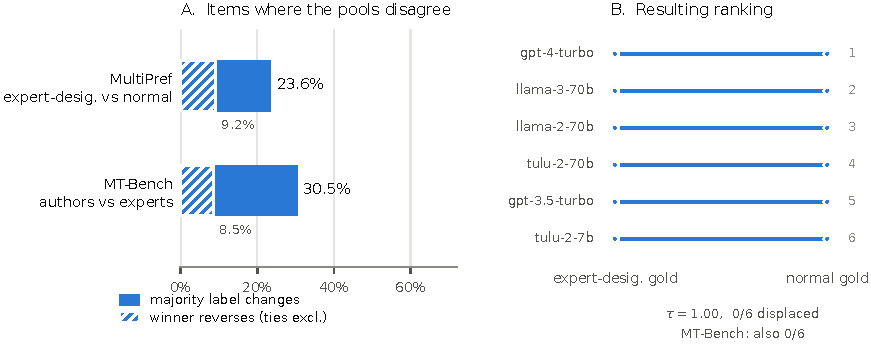
\includegraphics[width=0.96\textwidth]{fig1_divergence_vs_invariance.pdf}
\caption{Two pools annotating the same items disagree substantially
(\textbf{A}) and produce identical model rankings (\textbf{B}). Hatching marks
outright winner reversals, a strict subset of majority-label changes. Panel B
shows \textsc{MultiPref}; \textsc{MT-Bench} likewise displaces zero of six. Panel B is a
six-model leaderboard, and \S\ref{sec:threshold} shows that is doing much of the work: an
item-level bootstrap of the same corpus displaces a model in $28\%$ of resamples.}
\label{fig:main}
\end{figure}

\begin{table}[t]
\centering
\small
\caption{The same pattern on two corpora with different pool contrasts. Winner
reversal excludes ties on both sides, so it counts only items where both pools
name a decisive and opposite winner. \textsc{MultiPref} is restricted to items where both pools are
internally unanimous, and \textsc{MT-Bench} likewise, so no tie-breaking convention
enters either corpus.}
\label{tab:main}
\begin{tabular}{lccccc}
\toprule
Corpus & Pool contrast & Items & Majority differs & Winner reverses & Kendall $\tau$ \\
\midrule
\textsc{MultiPref} & expert-desig.\ vs.\ normal & $2{,}885$  & $23.6\%$ & $9.2\%$  & $1.0000$ \\
\textsc{MT-Bench}  & authors vs.\ experts & $246$      & $30.5\%$ & $8.5\%$  & $1.0000$ \\
\bottomrule
\end{tabular}
\end{table}

\begin{table}[t]
\centering
\small
\caption{Every tie-breaking convention we tried, on all $10{,}461$ \textsc{MultiPref}
comparisons (the unanimous row is the $2{,}885$-item subset, where no rule is consulted).
The first row is the rule our leaderboard actually used. Only the last, the rule ranking
A over Tie over B that our judge arm used (\S\ref{sec:judge}), moves the ranking; its mirror image does not, so the
ordering result depends on the aggregation convention. The last column is the correlation
between a pair's model-quality gap and its divergence rate: the convention decides even
the sign, and the flat reading belongs to the same rule the $\tau$ column isolates.}
\label{tab:tiebreak}
\begin{tabular}{lcccc}
\toprule
Tie-break rule & Majority differs & Winner reverses & Kendall $\tau$ (displaced) & $r$(gap) \\
\midrule
A $>$ B $>$ Tie (leaderboard)   & $44.9\%$ & $29.8\%$ & $1.0000$ ($0/6$) & $-0.081$ \\
Both pools unanimous (no rule)  & $23.6\%$ & $9.2\%$  & $1.0000$ ($0/6$) & $-0.154$ \\
Force ties to Tie               & $41.2\%$ & $2.5\%$  & $1.0000$ ($0/6$) & $+0.097$ \\
B $>$ Tie $>$ A (mirror)        & $36.6\%$ & $9.4\%$  & $1.0000$ ($0/6$) & $-0.220$ \\
A $>$ Tie $>$ B (judge arm)     & $49.8\%$ & $16.8\%$ & $0.4667$ ($4/6$) & $+0.030$ \\
\bottomrule
\end{tabular}
\end{table}

Table~\ref{tab:main} and Figure~\ref{fig:main} give the result. On
the convention-free \textsc{MultiPref} subset, one comparison in eleven has the two pools' majorities naming
opposite winners. Where the divergence sits is a convention-dependent question, so we answer it
under all of them. On the convention-free subset, bucketing items by the quality
gap between the two models compared gives $30.8\%$, $24.3\%$ and $15.3\%$ majority
divergence across tertiles, from the most closely matched pairs to the most widely
separated (Pearson $r = -0.154$). Across the five conventions of Table~\ref{tab:tiebreak} that
coefficient runs from $-0.220$ to $+0.097$ and \emph{changes sign}: it is negative under
three rules including the convention-free one, and positive under the other two. We
therefore do not claim that divergence concentrates on closely matched pairs, which would
be the convenient result here, since it is the adjacent pairs a displacement needs
(\S\ref{sec:threshold}). The tie-breaking rule decides even the sign of that relationship,
and one number that survives every convention is enough: divergence never falls below
$15.3\%$, even in the tertile of most widely separated model pairs.

The ordering is unchanged. Win rates move by $-2.1$ to $+2.8$pp and the rankings they
induce are identical: $\tau = 1.0000$, zero of six models displaced, on both corpora. The \textsc{MultiPref} bootstrap CI is
$[0.867, 1.000]$ and the \textsc{MT-Bench} CI is $[0.733, 1.000]$; the intervals
are wide because six models admit few discordant pairs, so we claim only that no
displacement occurs, not that none could.

A $9.2\%$ item-level reversal rate that leaves these orderings unchanged is still a $9.2\%$
reversal rate for any consumer that does not take the mean. But before drawing comfort from
the unchanged ordering, it is worth asking how much comfort six models can supply.

\section{How much invariance is that, exactly?}\label{sec:threshold}

A leaderboard can be invariant because aggregation is robust, or because nothing on it was
close enough to swap. Those are different claims and a $\tau$ of $1.00$ does not separate
them, so we measure the second directly.

\textbf{The perturbation.} Switching pools moves each model's win rate: across our six models
the normal-minus-expert-designated shift ranges from $-2.1$pp to $+2.8$pp, with
$\mathrm{SD} = 1.9$pp across models.

\begin{figure}[t]
\centering
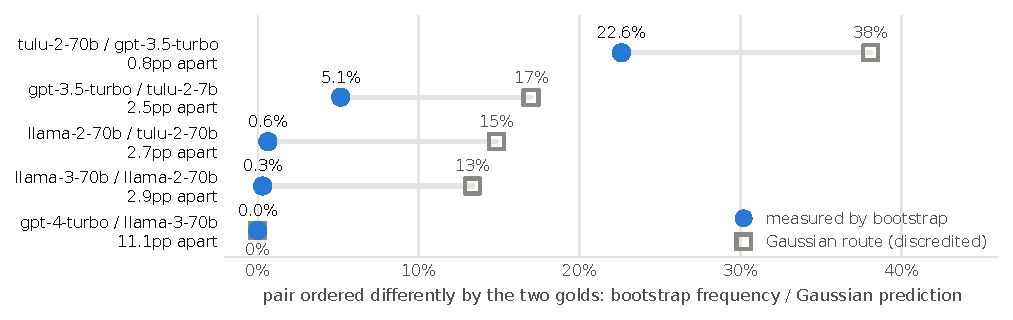
\includegraphics[width=\linewidth]{fig2_swap_by_gap.pdf}
\caption{Whole-leaderboard risk is concentrated in one adjacent pair, and the Gaussian
route over-predicts every pair with nonzero measured disagreement. Each row is an adjacent pair of the
\textsc{MultiPref} leaderboard, ordered by the gap between them; the filled circle is the
share of bootstrap resamples in which the two golds order that pair differently, the open
square is what the Gaussian approximation of \S\ref{sec:threshold} predicts for the same
pair. The approximation over-predicts all four nonzero pairs, which is why the section
reports it as failing rather than as a result.}
\label{fig:swapgap}
\end{figure}

\textbf{Our own leaderboard was lucky, and we measure how lucky rather than model it.} Its
adjacent gaps are $11.1$, $2.9$, $2.7$, $0.8$ and $2.5$pp. \textsc{MultiPref} reuses each
prompt for two comparisons against different model pairs, so the resampling unit is the
\emph{prompt} and a whole cluster travels together; $98.2\%$ of rows sit in a doubled prompt,
and resampling rows instead moves the rates below by less than a point. Resampling and
recomputing both leaderboards puts the whole-leaderboard displacement rate at $27.9\%$, and the closest
pair, $0.8$pp apart, is where almost all of it lives: the two golds order that pair
differently in $22.6\%$ of resamples, against $0.3$--$5.2\%$ for every other adjacent pair.
The observed zero is the modal outcome, not a reliable one.

A Gaussian route is available and we report it only to say that it does not work here.
Treating the two models' shifts as independent draws from the cross-model SD gives a pairwise
SD of $2.6$pp and a $38\%$ swap probability for the $0.8$pp pair, against the $22.6\%$
measured; for the three mid-sized gaps it predicts $13$--$17\%$ against $0.3$--$5.2\%$. The
error is in the input, not the algebra: $1.9$pp is the dispersion of six models' realised
shifts, whereas the quantity a swap depends on is the sampling SD of one \emph{pair's} shift
difference, which the bootstrap puts at $1.3$pp. Substituting that recovers the bootstrap
($32\%$ against $27.9\%$). The $2.6$pp input is therefore too large, and
Table~\ref{tab:threshold} is computed from it.

Appendix~\ref{app:sim} gives an illustrative simulation of larger boards; it is not
validated, and no claim in the paper rests on it.

This changes what the aggregate null licenses. It is not that leaderboards are robust to
who annotates. It is that \emph{this} six-model leaderboard, with one $11$pp gap in it and
one $0.8$pp gap that came up heads, survived, and that the item bootstrap on the very
same corpus fails to survive in $28\%$ of resamples. That much is measured. Whether the
reassurance also fails at larger $K$ is the extrapolation of Appendix~\ref{app:sim}, and it needs a corpus with
more models to settle. On a $20$-model board we would still stand behind the item-level
finding but not its exact rates, which describe these items, and behind neither
$\tau = 1.00$ nor the $28\%$, both specific to this board's spacing.

\section{What inherits the divergence}\label{sec:judge}

A widely deployed per-item consumer is the LLM judge, validated by
statements of the form \emph{``our judge agrees with humans $X\%$ of the time.''}
If a judge tracks one pool more than the other, $X$ is partly a statement about
the hiring decision. Neither pool is ground truth here: we measure which one a judge
tracks, not which one is right.

We judged a stratified sample of \textsc{MultiPref} with three local open-weight models,
in both presentation orders, under a schema-constrained five-point output identical to the
human scale. All three lean toward the normal pool under the three estimators of
Table~\ref{tab:judge}, all of which score against pool majorities tie-broken A over Tie
over B. That shared sign does not survive every way of collapsing a split pool
(\emph{Convention control}, below). How far is also a smaller and more fragile number than
our first draft of this section reported, for two reasons we now handle explicitly.

\paragraph{The sample is not the corpus.} Power to separate the pools lives almost entirely
in \emph{pool-split} items, where the two majorities disagree, so the sweep deliberately
drew $60\%$ of its $2{,}500$ items from that stratum against $49.8\%$ in the corpus. Any
agreement figure computed on the sample as drawn therefore overstates the corpus effect.
We reweight by the inverse sampling probability within each stratum, which is the estimand
a reader cares about (what the judge would have done on all $10{,}461$ comparisons),
and report that as primary. It shrinks each of the three effects by $17\%$.

\paragraph{One of three clears the bar at corpus weighting.} The pre-registered rule is
conjunctive: kill if the agreement difference \emph{and} the erasure difference are both
indistinguishable from zero. Reweighted to the corpus, Qwen3.6-27B clears it on agreement
($-3.5$pp, CI excluding zero) and Gemma-4 clears it on erasure ($+2.4$pp, CI excluding
zero), while Qwen3.6-35B-A3B clears neither ($-2.2$pp, CI $[-4.4, +0.1]$; erasure $+1.8$pp,
CI $[-0.2, +3.9]$) and would be killed under its own rule at that weighting. All three
point the same way under this tie-break and all three cleared the bar on the sample as
drawn, which is the sweep we pre-registered; we report the corpus-weighted numbers as
primary anyway, because the sample was chosen for power and not as an estimate of anything.
Three judges giving the same sign is weak evidence on its own: a sign test on three would
not reach significance. Holm-adjusting the six tests this bar involves, three judges by two
metrics, leaves only Qwen3.6-27B's agreement difference significant (adjusted $p = 0.016$,
from the prompt-level resampling below). Intervals outside this six-test family are
exploratory. Under this tie-break the summary is a consistent direction, a corpus-level
magnitude near $2$--$3.5$pp, and one judge that carries it individually.

On pool-split items, where the stratification does not bias a within-stratum share,
Qwen3.6-35B-A3B matches the normal pool on $46.3\%$, the expert-designated pool on $34.0\%$ and neither on
$19.7\%$; Qwen3.6-27B gives $40.6\%$, $32.7\%$ and $26.6\%$; Gemma-4 gives $39.5\%$,
$33.3\%$ and $27.2\%$. Among the items where the judge matched \emph{either} pool the normal-pool
share is $57.6\%$, $55.4\%$ and $54.3\%$.

\paragraph{Convention control.} The tie-break sets a pool's majority on roughly half the
corpus. To test whether the lean comes from that rule, or from the label marginals it
induces meeting a judge's own A/B response bias, we rescored the same saved calls under
every rule of Table~\ref{tab:tiebreak}, keeping the original strata and weights
(Table~\ref{tab:convention}). The sign is rule-dependent: under the leaderboard's rule, and
under B over Tie over A, Gemma-4's lean becomes $+0.5$pp. On the $214$ sampled items where
both pools are internally unanimous and disagree, the judges side with the
expert-designated pool $87$, $83$ and $90$ times and with the normal pool $83$, $83$ and
$79$ times. A per-annotator score, the judge's mean agreement with a pool's two annotators,
needs no tie-break and leaves a lean distinguishable from zero only for Qwen3.6-27B
($-2.5$pp, Holm-adjusted $p = 0.010$ across the three judges), whose original-rule lean
also exceeds what its label marginals predict; about half of Gemma-4's is what its
marginals predict.
These intervals resample whole prompts (Appendix~\ref{app:repro}); for the original rule
this leaves every corpus-weighted agreement and erasure interval on the same side of zero
as before. These checks
were added after review and are exploratory; they show that the published direction partly
reflects the aggregation rule, not what mechanism produces it.


We flag two honest complications, and a claim we are withdrawing on the strength of the
second. First, an initial run of the second model at half this sample size did \emph{not}
clear the pre-registered replication bar ($-0.8$pp, CI $[-4.4, +2.8]$, against $-4.2$pp at
full power under that same estimator); the effect appeared only once power was matched, and
we report that rather than presenting the matched run as the first attempt.

Second, we had explained the effect as attenuation by label noise, which predicts that a
cleaner judge shows a \emph{larger} effect. On the self-consistent subset the data ran
exactly the other way: order-swap direction reversal falls $44.6\% \to 24.5\% \to
23.7\%$ while the lean falls $6.9 \to 5.2 \to 3.7$pp. An earlier draft of this paper
offered that monotone pattern as the sharpest clue toward a replacement mechanism. It does
not survive the primary estimator. Reweighted to the corpus the three leans are $2.2$,
$3.5$ and $1.8$pp against those same inconsistency rates: not monotone, and the noisiest
judge is in the middle rather than at the top. The pattern was an artefact of the subset
itself. Conditioning on self-consistency keeps a different fraction of items for each
judge ($55\%$ for the most position-sensitive model against $76\%$ for the least), and
the items a judge is confident about are items where the pool lean is larger, so the
estimator rewards inconsistency with a bigger number. The attenuation explanation stays
withdrawn, its replacement is withdrawn too, and the mechanism is simply open.

\begin{figure}[t]
\centering
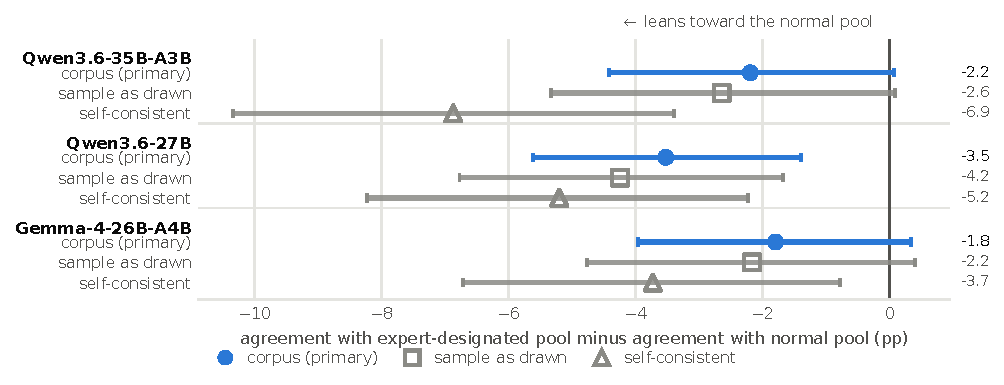
\includegraphics[width=\linewidth]{fig3_judge_forest.pdf}
\caption{Every judge leans toward the normal pool under all three estimators shown, which
share one tie-break (others: Table~\ref{tab:convention}). How far depends on which
estimator is designated primary. Points are the difference in agreement
with each pool, bars are $95\%$ bootstrap CIs, and the vertical line is no lean. Under the
corpus-reweighted estimator the paper treats as primary, one interval of three excludes
zero. The self-consistent subset sits systematically further from zero, which is the
artifact \S\ref{sec:judge} withdraws rather than a stronger result.}
\label{fig:judgeforest}
\end{figure}

\begin{table}[t]
\centering
\small
\caption{LLM-judge alignment with each annotator pool on \textsc{MultiPref}. Negative
means the judge agrees more with the \emph{normal} pool. \textbf{Corpus} is the primary
estimator: all items, midpoint order-combination, reweighted by inverse sampling
probability from the $60\%$ pool-split sample to the corpus's $49.8\%$; CIs are a
stratified paired bootstrap ($B=5000$). \textbf{Sample} is the same estimator on the sample
as drawn, and \textbf{Self-consistent} restricts to items where the judge gives the same
direction in both presentation orders, a pre-registered restriction that removes
uninformative items but also selects a different item set per judge, which is why it is
shown last rather than first. Every judge is negative under all three, which share the
A over Tie over B tie-break (Table~\ref{tab:convention}). $^{*}$ marks a CI
excluding zero. On the corpus estimator the erasure leg of the conjunctive bar is
$+1.8$pp $[-0.2, +3.9]$, $+2.0$pp $[-0.0, +4.0]$ and $+2.4$pp $[+0.3, +4.5]^{*}$ in table
order.}
\label{tab:judge}
\setlength{\tabcolsep}{2.5pt}
\footnotesize
\begin{tabular}{lccc}
\toprule
Judge & Corpus (primary) & Sample & Self-consistent \\
\midrule
Qwen3.6-35B-A3B (Qwen)   & $-0.022$ $[-0.044, +0.001]$     & $-0.026$ $[-0.053, +0.001]$     & $-0.069$ $[-0.103, -0.034]^{*}$ \\
Qwen3.6-27B (Qwen)       & $-0.035$ $[-0.056, -0.014]^{*}$ & $-0.042$ $[-0.068, -0.017]^{*}$ & $-0.052$ $[-0.082, -0.022]^{*}$ \\
Gemma-4-26B-A4B (Google) & $-0.018$ $[-0.040, +0.003]$     & $-0.022$ $[-0.048, +0.004]$     & $-0.037$ $[-0.067, -0.008]^{*}$ \\
\bottomrule
\end{tabular}
\end{table}

\begin{table}[t]
\centering
\small
\caption{Convention control: corpus-weighted agreement with the expert-designated pool minus
agreement with the normal pool, in pp, from the same saved calls, original strata and
weights. The first four columns tie-break each pool's majority differently; \emph{Per
annotator} needs no tie-break; \emph{Excess} is the original-rule difference minus its
expectation under independent labels within strata. $^{*}$ marks an unadjusted
prompt-resampled 95\% interval excluding zero (Appendix~\ref{app:repro}). Exploratory.}
\label{tab:convention}
\setlength{\tabcolsep}{4pt}
\begin{tabular}{lcccccc}
\toprule
Judge & A$>$Tie$>$B & A$>$B$>$Tie & B$>$Tie$>$A & Force Tie & Per annotator & Excess \\
\midrule
Qwen3.6-35B-A3B & $-2.2$ & $-1.8$ & $-1.0$ & $-2.7^{*}$ & $-1.6$ & $-2.0$ \\
Qwen3.6-27B & $-3.5^{*}$ & $-2.2^{*}$ & $-1.4$ & $-3.3^{*}$ & $-2.5^{*}$ & $-2.7^{*}$ \\
Gemma-4-26B-A4B & $-1.8$ & $+0.5$ & $+0.5$ & $-3.2^{*}$ & $-0.6$ & $-0.9$ \\
\bottomrule
\end{tabular}
\end{table}

\paragraph{Two further measurement choices move the judge more than the pool does.}
Both are by-products of the judge arm rather than targets of it, and both are far larger than
the $1.8$--$3.5$pp corpus-weighted pool effect the section is about, which is the reason to
record them. First, all three
judges are strongly position sensitive, reversing direction under order swap on
$44.6\%$, $24.5\%$ and $23.7\%$ of items, consistent with published position-bias
measurements \citep{positionbias2026} and, importantly, differing by a factor of
$1.8$ between the two Qwen models despite being the same family. Second, holding task content, model,
items, presentation orders, temperature and seed fixed while changing the output-format
instruction and its decoding constraint together (a JSON object versus a bare constrained
token), the same judge agrees with itself on only $47.2\%$ of items
$(n=500)$, with a systematic shift in one direction ($146$ items move A$\to$B, $3$
move B$\to$A). Judge numbers are conditional on output format, a
sensitivity of the kind \citet{judgesense2026} finds largely unexamined. Appendix~\ref{app:prompt} reports a partial localisation of this effect.

\section{What to do instead}

\textbf{Report the pool and the aggregation rule.} An LLM-judge agreement figure without
the annotator pool that defines its reference labels, and the rule that collapses a split
pool into one label, is under-specified by roughly the size of the effect being reported.

\textbf{Do not infer per-item reliability from leaderboard stability.} These are
different quantities and our data separates them by a wide margin. Nor should a
leaderboard's stability be read off the leaderboard itself: at six models the $\tau=1.00$
is partly a statement about how far apart the models were, and the item-level bootstrap in
\S\ref{sec:threshold} is the cheap check that says so.

\textbf{Counterbalance order, always.} At $23.7$--$44.6\%$ direction reversal, a
single-order judge measurement on this task is unstable on about a quarter to nearly half
of its items.

\textbf{Weight the sample you drew, and report the unrestricted estimator.} Stratifying a
judge sweep toward the items that carry the signal is the right way to spend inference, and
it makes every raw agreement rate a statement about the sample rather than the corpus;
reweighting cost us $17\%$ of the effect. The larger cost came from elsewhere: restricting
to items where the judge is self-consistent makes all three effects roughly double and all
three CIs exclude zero, and it keeps a different item set for each judge. Report the
unrestricted estimator first and the restriction as a sensitivity analysis, not the other
way round.

\textbf{Assign populations, not just annotators.} Per-annotator labels are necessary and
not sufficient: \textsc{PRISM} keeps rich participant profiles and
\textsc{HelpSteer2-Preference} keeps multiple annotators per item, and neither provides
systematic predefined-pool assignment: the first because one participant sees each conversation, the second
because there is no population split to condition on. A corpus that assigns two named
populations to the same items, as \textsc{MultiPref} does, is what makes the hiring
decision auditable after the fact.

\section{Limitations}\label{sec:limits}

Both corpora rank only six models. The aggregate invariance is therefore a statement
about this leaderboard's spacing, and \S\ref{sec:threshold} measures rather than asserts
what that costs by bootstrapping the same corpus. The $K > 6$ rows of
Table~\ref{tab:threshold} are a different kind of object and we label them as such
throughout: they extrapolate from six observed shifts under assumptions (i.i.d.\
Gaussian shifts across models, uniform spacing across the observed span) that six models
cannot check, and they are not bounds. Their agreement with the $K=6$ bootstrap is not a
validation either: Appendix~\ref{app:sim} withdraws that claim, having found it to be two
compensating errors that cancel at $K=6$ under uniform spacing and nowhere else. A corpus with $20$ or more models rated by two predefined
pools would settle the question directly and is the single experiment that would most
improve this paper. The \textsc{MT-Bench} contrast rests on $246$ convention-free cells of $292$
doubly-rated ones. The judge arm spans two vendors: \textsc{Laguna S 2.1} does not load in our stack, and a
substitute prefill path reproduced the generation path on $94.6\%$ of items against a
pre-registered $95\%$ bar, so we ran a third judge from a different pretraining lineage
instead, at the same Q8\_0 precision as the other two. That third judge is not a controlled
vendor swap, because architecture, pretraining corpus and post-training all change with
the lineage. It is a replication across three unlike systems rather than an isolation of
any one factor, and unlike systems may be less independent than a vendor count suggests:
in a different setting, $24$ open-weight monitors scoring backdoored code, a monitor's
agreement with the rest of its pool tracks its own detection skill (Spearman $0.84$)
rather than its pretraining lineage ($+0.064$, $p = 0.18$) \citep{jha2026decorrelation}. Under the original tie-break the normal-pool lean holds in
sign across all three, but at corpus weighting only one of the three has an agreement CI
excluding zero, a consistent sign across three judges is not itself significant, and for one
judge the sign depends on the rule. Three models from two vendors is not a claim about
judges in general. A fourth judge or a reward-model probe would widen the sample but not
settle which aggregation rule defines the reference label, which the convention control
addresses. We report the null, the failed under-powered run, and the withdrawn
explanation alongside the positive results deliberately: the paper's claim is
about measurement validity, and it would be self-undermining to present it
selectively. All local judge inference ran on a single on-premises NVIDIA GB10
(Grace Blackwell) workstation serving Q8\_0-quantised GGUF checkpoints; the three
judge sweeps (2{,}500 comparisons $\times$ 2 presentation orders each) took
49--122 minutes wall-clock per model.

\section{Related work}

\paragraph{The closest work.} \citet{zhang2025diverging} is the paper this one has to
be measured against. They analyse disagreement in \textsc{MultiPref} and
\textsc{HelpSteer2}, build a ten-category taxonomy of its causes, establish that most
disagreement reflects genuine differences in taste rather than annotation error, release
\textsc{MultiPref}-Disagreements, and show that Bradley--Terry reward models and
LLM-as-Judge evaluation both fail to represent divergent annotators. Everything in this
paper about \emph{whether} \textsc{MultiPref} annotators disagree is downstream of that
result, not a discovery of ours, and our $50.1\%$ within-pool figure is a recomputation in
their territory. Two things separate the papers. Their unit is the annotator pair, taken
over all permutations of the four annotators on an item, which averages across the
normal/expert designation; ours is the \emph{pool}, held fixed by
\textsc{MultiPref}'s own assignment, which is the contrast its authors named as future work
and the one Zhang et al.\ marginalise over. And they do not follow disagreement into a
model ranking: there is no leaderboard or Kendall $\tau$ analysis in their paper, whose
win/loss/tie rates compare response types under an LLM judge, so the question of whether
pool choice reaches the thing benchmarks actually report is open after it and answered here
only for two six-model boards.

\paragraph{The rest.} Perspectivist evaluation argues that annotator disagreement is signal
rather than noise \citep{perspectivist2026}. \textsc{StableVal} \citep{stableval2026} is
the nearest antecedent on the aggregate side: it models annotator confusion and reports
that majority vote yields ranking \emph{instability} under annotator heterogeneity, where
we find a stable ranking under a specific, pre-assigned heterogeneity.
\citet{kadekodi2025selective} take the other route open to an aggregator, abstaining from
comparisons where fewer than a chosen fraction of individuals agree and returning a partial
order rather than arbitrating dissent; that is a safer rule for a fixed set of voters, where
we ask the prior question of which population supplies them. These results are
compatible: our finding concerns two particular recruited populations and six-model
leaderboards, and our own bootstrap displaces a model in $28\%$ of resamples. But a reader
should treat \textsc{StableVal}'s finding, not ours, as the general statement about
majority vote. Work on LLM-judge
bias documents position effects \citep{positionbias2026} and instability under
semantically equivalent prompt rephrasings \citep{judgesense2026}; our position numbers
replicate that line rather than extend it, and our format numbers are reported alongside
them as controls on the pool measurement.

\bibliographystyle{plainnat}
\begin{thebibliography}{9}
\small
\bibitem[Miranda et al.(2024)]{miranda2024hybrid} L.~Miranda et al.
\newblock Hybrid Preferences: Learning to Route Instances for Human vs.\ AI Feedback.
\newblock \href{https://arxiv.org/abs/2410.19133}{\emph{arXiv:2410.19133}}, 2024.
\bibitem[Zheng et al.(2023)]{zheng2023judging} L.~Zheng et al.
\newblock Judging LLM-as-a-Judge with MT-Bench and Chatbot Arena.
\newblock \emph{NeurIPS Datasets and Benchmarks}, 2023.
\newblock \href{https://arxiv.org/abs/2306.05685}{arXiv:2306.05685}.
\bibitem[Kirk et al.(2024)]{kirk2024prism} H.~R.~Kirk et al.
\newblock The PRISM Alignment Dataset.
\newblock \emph{NeurIPS Datasets and Benchmarks}, 2024.
\newblock \href{https://arxiv.org/abs/2404.16019}{arXiv:2404.16019}.
\bibitem[Wang et al.(2024a)]{wang2024helpsteer2} Z.~Wang et al.
\newblock HelpSteer2: Open-source dataset for training top-performing reward models.
\newblock \href{https://arxiv.org/abs/2406.08673}{\emph{arXiv:2406.08673}}, 2024.
\bibitem[Wang et al.(2024b)]{wang2024helpsteer2pref} Z.~Wang et al.
\newblock HelpSteer2-Preference: Complementing ratings with preferences.
\newblock \href{https://arxiv.org/abs/2410.01257}{\emph{arXiv:2410.01257}}, 2024.
\bibitem[Zhang et al.(2025)]{zhang2025diverging} M.~J.~Q. Zhang, Z.~Wang, J.~D. Hwang,
Y.~Dong, O.~Delalleau, Y.~Choi, E.~Choi, X.~Ren, and V.~Pyatkin.
\newblock Diverging preferences: When do annotators disagree and do models know?
\newblock \emph{ICML}, 2025.
\newblock \href{https://arxiv.org/abs/2410.14632}{arXiv:2410.14632}.
\bibitem[Xu and Jurgens(2026)]{perspectivist2026} Y.~Xu and D.~Jurgens.
\newblock Beyond consensus: Perspectivist modeling and evaluation of annotator disagreement in NLP.
\newblock \href{https://arxiv.org/abs/2601.09065}{\emph{arXiv:2601.09065}}, 2026.
\bibitem[Bonagiri et al.(2026)]{stableval2026} A.~Bonagiri et al.
\newblock STABLEVAL: Disagreement-aware and stable evaluation of AI systems.
\newblock \href{https://arxiv.org/abs/2605.02122}{\emph{arXiv:2605.02122}}, 2026.
\bibitem[Kadekodi et al.(2025)]{kadekodi2025selective} S.~Kadekodi, H.~Mctavish, and B.~Ustun.
\newblock Selective preference aggregation.
\newblock In \emph{ICML}, volume~267 of \emph{PMLR}, pages 28644--28669, 2025.
  \url{https://proceedings.mlr.press/v267/kadekodi25a.html}.
\bibitem[Jha(2026)]{jha2026decorrelation} A.~Jha.
\newblock Decorrelation is not complementarity: Skill, not lineage, governs
  trusted-monitor ensembles.
\newblock \href{https://arxiv.org/abs/2608.16190}{\emph{arXiv:2608.16190}}, 2026.
\bibitem[Mazur(2026)]{positionbias2026} L.~Mazur.
\newblock LLM judge position-bias benchmark.
\newblock \url{https://github.com/lechmazur/position_bias}, 2026. Accessed 2026-08-16.
\bibitem[Bellibatlu et al.(2026)]{judgesense2026} R.~R.~Bellibatlu, E.~Raff, and W.~Zhang.
\newblock JudgeSense: A benchmark for prompt sensitivity in LLM-as-a-judge systems.
\newblock \href{https://arxiv.org/abs/2604.23478}{\emph{arXiv:2604.23478}}, 2026.
\end{thebibliography}

\appendix
\section{Larger boards: an illustration, not a measurement}\label{app:sim}

\textbf{What that would mean for a larger board, if the perturbation carried over.} The
question a reader asks next is what happens at the leaderboard sizes the field actually
publishes, and we can only answer it by extrapolation, so we mark it as one.
Table~\ref{tab:threshold} holds the measured shift distribution fixed, assumes those
shifts are i.i.d.\ Gaussian across models, spreads $K$ models uniformly over the observed
win-rate span, and simulates. Displacement probability rises from $0.29$ at $K=6$ to
$0.92$ at $K=10$ and to $1.00$ by $K=20$.

Three cautions, because the arithmetic is much more confident than the evidence under it. The
shift distribution is estimated from \emph{six} models, so its SD is itself poorly determined.
Independence across models is assumed and, on the evidence above, wrong: the measured
pairwise SD is half what independence implies. And uniform spacing over one corpus's
observed span is a stipulation about a hypothetical leaderboard, not a fact about any real one.
An earlier draft of this paper offered the $K=6$ row as a validation, since the simulation's
$0.293$ sits next to the item bootstrap's $0.279$. That agreement is a coincidence of two
compensating errors and we withdraw the claim: run the identical simulation on the
\emph{observed} gaps rather than uniform ones and it returns $0.70$ against the same measured
$0.28$. Uniform spacing is more forgiving than this board's real gap structure, and the
$2.6$pp input is roughly twice the measured pairwise SD; the two cancel at $K=6$ uniform and
nowhere else. Table~\ref{tab:threshold} is therefore an illustration of what a
\emph{mis-calibrated} perturbation would imply. Its two errors push in opposite
directions: the inflated $2.6$pp input upward, uniform spacing downward against this board's
real gaps. We therefore do not claim to know the net direction of the $K>6$ rows, and no row
of it is checked.

\begin{table}[ht]
\centering
\small
\caption{\textbf{An illustrative scenario, not a measurement.} Probability that changing
the annotator pool displaces at least one model, holding the measured per-model shift
($\mathrm{SD} = 1.9$pp) fixed, assuming those shifts are i.i.d.\ Gaussian across models,
and spreading $K$ models uniformly across the observed win-rate span. Probabilities are
Monte Carlo over per-model shifts ($2\times10^{5}$ draws), so adjacent pairs correctly
share a model; the closed form $1-(1-p)^{K-1}$ used in an earlier draft treats the $K-1$
swap events as independent, which they are not, and understates $K=10$ by $5$pp. \textbf{No
column here is validated.} The $K=6$ row sits close to the item bootstrap's $0.279$ only
because uniform spacing happens to offset an inflated shift SD; on the observed gaps the same
simulation returns $0.70$. Read the column as an illustration, not as a bound.}
\label{tab:threshold}
\begin{tabular}{lccccc}
\toprule
Models on the leaderboard & 6 & 10 & 20 & 30 & 50 \\
\midrule
Gap between adjacent models & $4.0$pp & $2.2$pp & $1.1$pp & $0.7$pp & $0.4$pp \\
P(at least one displaced)   & $0.29$  & $0.92$  & $1.00$ & $1.00$ & $1.00$ \\
\bottomrule
\end{tabular}
\end{table}

\section{Reproduction details}\label{app:repro}

Code, results files, per-call judge outputs, a label-only \textsc{MultiPref} derivative
(identifiers and A/Tie/B labels, no prompt or response text) and excerpts of the
decision-rule ledger are released at \url{https://github.com/anik-jha/whose-gold}. The
leaderboard analyses rerun from the public corpora, the convention control replays from the
saved judge calls without model inference, and a verifier script checks $106$ of the
reported numbers against their results files. Regenerating the judge calls requires the three checkpoints named
below and a \texttt{llama.cpp} server.

The stratified sample is $2{,}500$ items drawn with
\texttt{numpy} PCG64 seed $17$, $60\%$ from the pool-split stratum, from the $10{,}461$
\textsc{MultiPref} comparisons carrying both pools; the same draw is reused for every
judge. The reweighting in Table~\ref{tab:judge} of \S\ref{sec:judge} gives each scored item the weight
$N_{\text{stratum}}/n_{\text{stratum}}$, where $n$ is that judge's \emph{scored} count in the
stratum rather than the drawn count, since a handful of items fail to parse
($5210/1498$ and $5251/998$ for the first two judges, $5210/1497$ and $5251/998$ for the
third). Judges are served by \texttt{llama.cpp} at Q8\_0 from
\texttt{Qwen\_Qwen3.6-35B-A3B-Q8\_0.gguf},
\texttt{Qwen\_Qwen3.6-27B-Q8\_0.gguf} and
\texttt{google\_\_gemma-4-26b-a4b-it-Q8\_0.gguf}, temperature $0$, server seed $1234$, with
output constrained to the JSON schema
\texttt{\{"p": <"1".."5">\}} whose five codes are the five points of the human preference
scale; the format-sensitivity check replaces it with the grammar
\texttt{root ::= [1-5]}. Every item is issued in both presentation orders and combined at
the midpoint. Bootstraps are $B=5000$ (corpus and sample-as-drawn judge estimates, seed
$0$), $B=10{,}000$ (self-consistent judge estimates, seed $17$), $B=2000$ (leaderboard
$\tau$ intervals, seed $0$) and $B=4000$ (displacement analysis, seed $0$); the convention
control resamples whole prompts, since $604$ of each judge's scored rows share a prompt:
each prompt draws one mean-one exponential weight, shared across strata and judges, and
each stratum is renormalized to its corpus mass ($5{,}000$ replicates, seed $20261002$).
The illustrative
$K$-model simulation uses $2\times10^{5}$ draws.

For the convention control we report percentile 95\% intervals and approximate two-sided
centered-multiplier $p$-values, $(1 + \#\{b : |\hat\theta_b - \hat\theta| \ge |\hat\theta|\})/(B + 1)$.
This is an exploratory sensitivity analysis for a superpopulation of independent prompts,
conditional on the original stratum masses; it is not exact inference under the
finite-population sampling design, and dependence through repeated annotators is not
modelled. The stars in Table~\ref{tab:convention} use these intervals without adjustment.
Holm adjustment is applied separately to two exploratory families: the six original-rule
agreement and erasure tests of \S\ref{sec:judge}, and the three per-annotator tests. The
per-annotator differences and intervals, in pp and table order, are $-1.6$ $[-3.23, +0.17]$,
$-2.5$ $[-4.02, -0.81]$ and $-0.6$ $[-2.27, +1.05]$.

\section{Judge prompt}\label{app:prompt}

The system prompt below is the one the sweep served, verbatim. The paper shows that judge
output is highly sensitive to the response format (\S\ref{sec:judge}), which makes the exact
string load-bearing rather than incidental, so it is reproduced here rather than left to the
code release. Decoding is constrained to the JSON schema \verb|{"p": <"1".."5">}|. The
format-sensitivity check of \S\ref{sec:judge} replaces both the constraint, with the grammar
\verb|root ::= [1-5]|, and the final sentence of the system prompt, which becomes
\verb|Reply with exactly one digit and nothing else:| in place of the JSON instruction. Those
two change together, which is why \S\ref{sec:judge} does not attribute the effect to the
scaffolding alone. Everything else is identical.

\begin{verbatim}
You are evaluating two candidate responses to a user's message. Judge which
response is better overall, considering helpfulness, truthfulness, and
harmlessness. Reply with JSON {"p": "<code>"} using this scale:
  1 = A-is-clearly-better
  2 = A-is-slightly-better
  3 = Tie
  4 = B-is-slightly-better
  5 = B-is-clearly-better
\end{verbatim}

\noindent The user message is templated as:

\begin{verbatim}
User's message:
{prompt}

--- Response A ---
{a}

--- Response B ---
{b}

Which response is better overall?
\end{verbatim}

\noindent Each field is clipped from the middle to 6{,}000 characters, keeping both ends.
Every item is issued in both presentation orders; in order \texttt{ba} the two completions
are swapped before templating.

\noindent The format effect of \S\ref{sec:judge} can be partly localised: re-scoring the same
items with the same model at bf16 (rather than the Q8\_0 quantisation the sweep
served) by \emph{prefilling} the JSON scaffolding and reading the next-token
distribution recovers $94.6\%$ agreement with the generated labels, against
$47.2\%$ for a bare digit. That check is not clean: it changes precision (bf16 against Q8\_0) and decoding path
(prefill against generation) at the same time, so the $5.4\%$ residual absorbs both and we
cannot separate them. The prefill check thus disagrees with the generated labels on
$5.4\%$ of items, against $52.8\%$ for the JSON-versus-digit condition.
That condition is itself compound: it changes the system's output-format instruction as well
as the decoding constraint, so this audit cannot separate instruction wording from JSON
scaffolding. A clean attribution needs the constraint varied at fixed instruction wording,
fixed precision and fixed decoding path, which we did not run.


\newpage
\section*{NeurIPS Paper Checklist}

\begin{enumerate}

\item {\bf Claims}
    \item[] Question: Do the main claims made in the abstract and introduction accurately reflect the paper's contributions and scope?
    \item[] Answer: \answerYes{}
    \item[] Justification: The abstract and introduction state the measured claims (item-level divergence between predefined pools, leaderboard invariance at $K=6$ with the $28\%$ bootstrap displacement rate alongside it, and the corpus-reweighted judge lean with its one-of-three significance and its dependence on the tie-break rule) and explicitly separate what is measured from what is conjectured (contribution 3); Table~\ref{tab:summary} labels the evidence behind each headline number. The $K>6$ rows of Table~\ref{tab:threshold} are an extrapolation and are labelled as an illustrative scenario in the section, the table caption and the Limitations rather than reported as probabilities the data establish; they are not used to support any claim. Section~\ref{sec:limits} states the scope bounds (six-model corpora, three judges from two vendors, a judge lean whose sign depends on the aggregation rule) that the abstract's language is written to respect.
    \item[] Guidelines:
    \begin{itemize}
        \item The answer \answerNA{} means that the abstract and introduction do not include the claims made in the paper.
        \item The abstract and/or introduction should clearly state the claims made, including the contributions made in the paper and important assumptions and limitations. A \answerNo{} or \answerNA{} answer to this question will not be perceived well by the reviewers.
        \item The claims made should match theoretical and experimental results, and reflect how much the results can be expected to generalize to other settings.
        \item It is fine to include aspirational goals as motivation as long as it is clear that these goals are not attained by the paper.
    \end{itemize}

\item {\bf Limitations}
    \item[] Question: Does the paper discuss the limitations of the work performed by the authors?
    \item[] Answer: \answerYes{}
    \item[] Justification: Section~\ref{sec:limits} (Limitations) discusses the leaderboard-size dependence of the aggregate-invariance claim, the Gaussian and independence assumptions behind the threshold extrapolation, the corpus sizes behind each contrast, the two-vendor bound on the judge claim, and reports the null, the underpowered failed run, and the withdrawn attenuation hypothesis alongside the positive results.
    \item[] Guidelines:
    \begin{itemize}
        \item The answer \answerNA{} means that the paper has no limitation while the answer \answerNo{} means that the paper has limitations, but those are not discussed in the paper.
        \item The authors are encouraged to create a separate ``Limitations'' section in their paper.
        \item The paper should point out any strong assumptions and how robust the results are to violations of these assumptions.
        \item The authors should reflect on the scope of the claims made, e.g., if the approach was only tested on a few datasets or with a few runs.
        \item The authors should reflect on the factors that influence the performance of the approach.
        \item The authors should discuss the computational efficiency of the proposed algorithms and how they scale with dataset size.
        \item If applicable, the authors should discuss possible limitations of their approach to address problems of privacy and fairness.
        \item Reviewers will be specifically instructed to not penalize honesty concerning limitations.
    \end{itemize}

\item {\bf Theory assumptions and proofs}
    \item[] Question: For each theoretical result, does the paper provide the full set of assumptions and a complete (and correct) proof?
    \item[] Answer: \answerNA{}
    \item[] Justification: The paper contains no theorems. The displacement-probability extrapolation of Appendix~\ref{app:sim} is an empirical statistical estimate under a stated Gaussian, uniform-spacing approximation, not a proof and not validated: the section withdraws the one agreement that had been offered as a check on it, and states that no row of the table is checked.
    \item[] Guidelines:
    \begin{itemize}
        \item The answer \answerNA{} means that the paper does not include theoretical results.
        \item All the theorems, formulas, and proofs in the paper should be numbered and cross-referenced.
        \item All assumptions should be clearly stated or referenced in the statement of any theorems.
    \end{itemize}

\item {\bf Experimental result reproducibility}
    \item[] Question: Does the paper fully disclose all the information needed to reproduce the main experimental results of the paper to the extent that it affects the main claims and/or conclusions of the paper (regardless of whether the code and data are provided or not)?
    \item[] Answer: \answerYes{}
    \item[] Justification: Setup states corpus identities and sizes, the aggregation and tie-break rule with its full sensitivity table, and the paired-bootstrap procedure. Appendix~\ref{app:repro} gives the sampling seed and stratum fractions, the stratum weights used for reweighting, the exact GGUF checkpoint filenames and serving precision, the decoding temperature and server seed, the constrained output schema and the grammar used for the format check, the order-combination rule, and every bootstrap size and seed. All corpora are public and named with their citations. Appendix~\ref{app:prompt} reproduces the judge system prompt and user template verbatim, which the paper's own format-sensitivity result makes load-bearing rather than incidental.
    \item[] Guidelines:
    \begin{itemize}
        \item The answer \answerNA{} means that the paper does not include experiments.
        \item If the paper includes experiments, a \answerNo{} answer to this question will not be perceived well by the reviewers.
        \item If the contribution is a dataset and/or model, the authors should describe the steps taken to make their results reproducible or verifiable.
    \end{itemize}

\item {\bf Open access to data and code}
    \item[] Question: Does the paper provide open access to the data and code, with sufficient instructions to faithfully reproduce the main experimental results, as described in supplemental material?
    \item[] Answer: \answerYes{}
    \item[] Justification: Code, results files, per-call judge outputs, a label-only \textsc{MultiPref} derivative and decision-rule ledger excerpts are at \url{https://github.com/anik-jha/whose-gold}, with instructions. The leaderboard analyses rerun from the public corpora (\textsc{MultiPref}, \textsc{MT-Bench}), the convention control replays offline from the saved judge calls, and a verifier script checks $106$ of the reported numbers against their results files. Regenerating the judge calls requires the GGUF checkpoints named in Appendix~\ref{app:repro}.
    \item[] Guidelines:
    \begin{itemize}
        \item The answer \answerNA{} means that paper does not include experiments requiring code.
        \item While we encourage the release of code and data, we understand that this might not be possible, so \answerNo{} is an acceptable answer.
        \item At submission time, to preserve anonymity, the authors should release anonymized versions (if applicable).
    \end{itemize}

\item {\bf Experimental setting/details}
    \item[] Question: Does the paper specify all the training and test details (e.g., data splits, hyperparameters, how they were chosen, type of optimizer) necessary to understand the results?
    \item[] Answer: \answerYes{}
    \item[] Justification: Setup and Section~\ref{sec:judge} give sample sizes, the judge output schema, the models and their serving precision, the stratification into pool-split/pool-agree strata, and the pre-registered sample size and bar per judge.
    \item[] Guidelines:
    \begin{itemize}
        \item The answer \answerNA{} means that the paper does not include experiments.
        \item The experimental setting should be presented in the core of the paper to a level of detail that is necessary to appreciate the results and make sense of them.
    \end{itemize}

\item {\bf Experiment statistical significance}
    \item[] Question: Does the paper report error bars suitably and correctly defined or other appropriate information about the statistical significance of the experiments?
    \item[] Answer: \answerYes{}
    \item[] Justification: Every \emph{inferential} headline number carries a 95\% CI from a paired or item-level bootstrap (Kendall $\tau$ CIs in Section~3, judge agreement and erasure differences in Table~\ref{tab:judge}, and prompt-resampled intervals for the exploratory controls, starred in Table~\ref{tab:convention} and given for the per-annotator estimator in Appendix~\ref{app:repro}), and the paper states the bootstrap procedure and sample sizes behind each. The judge-arm tests are Holm-adjusted where stated, and Table~\ref{tab:summary} separates measured, primary and exploratory results. The divergence rates in Table~\ref{tab:main} and the tie-break sensitivities in Table~\ref{tab:tiebreak} are exact descriptive counts over a fixed, fully observed corpus rather than estimates of a sampling distribution, so they are reported without intervals; the displacement rates in Section~\ref{sec:threshold} are themselves bootstrap frequencies. Table~\ref{tab:threshold} is labelled throughout as an illustrative simulation and is not a measurement, so no interval is attached to it.
    \item[] Guidelines:
    \begin{itemize}
        \item The answer \answerNA{} means that the paper does not include experiments.
        \item The authors should answer \answerYes{} if the results are accompanied by error bars, confidence intervals, or statistical significance tests, at least for the experiments that support the main claims of the paper.
        \item The method for calculating the error bars should be explained.
    \end{itemize}

\item {\bf Experiments compute resources}
    \item[] Question: For each experiment, does the paper provide sufficient information on the computer resources (type of compute workers, memory, time of execution) needed to reproduce the experiments?
    \item[] Answer: \answerYes{}
    \item[] Justification: Limitations states the hardware (a single on-premises NVIDIA GB10 workstation with 119\,GB of unified CPU+GPU memory), the serving precision (Q8\_0 GGUF, the largest checkpoint resident at roughly 37\,GB), and the wall-clock range (49--122 minutes per judge sweep) for the only GPU-bound stage. All other analysis is CPU-only and runs in minutes; the raw per-call judge outputs are under 1\,GB.
    \item[] Guidelines:
    \begin{itemize}
        \item The answer \answerNA{} means that the paper does not include experiments.
        \item The paper should indicate the type of compute workers CPU or GPU, internal cluster, or cloud provider, including relevant memory and storage.
        \item The paper should disclose whether the full research project required more compute than the experiments reported in the paper.
    \end{itemize}

\item {\bf Code of ethics}
    \item[] Question: Does the research conducted in the paper conform, in every respect, with the NeurIPS Code of Ethics \url{https://neurips.cc/public/EthicsGuidelines}?
    \item[] Answer: \answerYes{}
    \item[] Justification: The paper reanalyzes existing, publicly released annotation data and runs open-weight models locally; it collects no new human-subjects data and introduces no new deployment or dual-use risk.
    \item[] Guidelines:
    \begin{itemize}
        \item The answer \answerNA{} means that the authors have not reviewed the NeurIPS Code of Ethics.
        \item If the authors answer \answerNo, they should explain the special circumstances that require a deviation from the Code of Ethics.
    \end{itemize}

\item {\bf Broader impacts}
    \item[] Question: Does the paper discuss both potential positive societal impacts and negative societal impacts of the work performed?
    \item[] Answer: \answerYes{}
    \item[] Justification: Positive: the paper argues for reporting the annotator pool behind any human-agreement figure, which makes evaluation claims auditable. Negative, and the reason this is not purely upside: a demonstration that the choice of annotator population moves item-level labels can be used to \emph{select} a pool that produces a favourable number, which is benchmark gaming with a methodological alibi. The same finding can also be misread as licence to dismiss annotators whose labels are inconvenient, or to treat the expert-designated pool as correct when our data give no basis for calling either pool the ground truth. We state explicitly (\S\ref{sec:judge}) that neither pool is ground truth and that the paper measures divergence rather than adjudicating it.
    \item[] Guidelines:
    \begin{itemize}
        \item The answer \answerNA{} means that there is no societal impact of the work performed.
        \item Examples of negative societal impacts include fairness considerations (e.g., deployment of technologies that could make decisions that unfairly impact specific groups).
    \end{itemize}

\item {\bf Safeguards}
    \item[] Question: Does the paper describe safeguards that have been put in place for responsible release of data or models that have a high risk for misuse?
    \item[] Answer: \answerNA{}
    \item[] Justification: The paper releases no model and no scraped dataset; it analyzes existing public benchmarks and open-weight models used only as judges.
    \item[] Guidelines:
    \begin{itemize}
        \item The answer \answerNA{} means that the paper poses no such risks.
    \end{itemize}

\item {\bf Licenses for existing assets}
    \item[] Question: Are the creators or original owners of assets (e.g., code, data, models), used in the paper, properly credited and are the license and terms of use explicitly mentioned and properly respected?
    \item[] Answer: \answerNo{}
    \item[] Justification: \textsc{MultiPref}, \textsc{MT-Bench} human judgments, \textsc{PRISM}, and \textsc{HelpSteer2}/\textsc{HelpSteer2-Preference} are credited via citation and the judge checkpoints are named exactly, but license names and terms are not enumerated in the text. We answer No rather than asserting licenses we have not each individually re-checked.
    \item[] Guidelines:
    \begin{itemize}
        \item The answer \answerNA{} means that the paper does not use existing assets.
        \item The authors should cite the original paper that produced the code package or dataset.
        \item The name of the license (e.g., CC-BY 4.0) should be included for each asset.
    \end{itemize}

\item {\bf New assets}
    \item[] Question: Are new assets introduced in the paper well documented and is the documentation provided alongside the assets?
    \item[] Answer: \answerYes{}
    \item[] Justification: No new model is created. The release's derived assets, the per-call judge outputs and a label-only \textsc{MultiPref} derivative (identifiers and A/Tie/B labels, no prompt or response text), are documented in its README and asset notes, which give upstream attribution and licenses.
    \item[] Guidelines:
    \begin{itemize}
        \item The answer \answerNA{} means that the paper does not release new assets.
        \item At submission time, remember to anonymize your assets (if applicable).
    \end{itemize}

\item {\bf Crowdsourcing and research with human subjects}
    \item[] Question: For crowdsourcing experiments and research with human subjects, does the paper include the full text of instructions given to participants and screenshots, if applicable, as well as details about compensation (if any)?
    \item[] Answer: \answerNA{}
    \item[] Justification: This paper conducts no new crowdsourcing or human-subjects research; it reanalyzes annotations already collected and released by \textsc{MultiPref} and \textsc{MT-Bench}, whose own papers document their annotation instructions and compensation.
    \item[] Guidelines:
    \begin{itemize}
        \item The answer \answerNA{} means that the paper does not involve crowdsourcing nor research with human subjects.
    \end{itemize}

\item {\bf Institutional review board (IRB) approvals or equivalent for research with human subjects}
    \item[] Question: Does the paper describe potential risks incurred by study participants, whether such risks were disclosed to the subjects, and whether Institutional Review Board (IRB) approvals (or an equivalent approval/review) were obtained?
    \item[] Answer: \answerNA{}
    \item[] Justification: No new human-subjects research was conducted; see the previous item.
    \item[] Guidelines:
    \begin{itemize}
        \item The answer \answerNA{} means that the paper does not involve crowdsourcing nor research with human subjects.
    \end{itemize}

\item {\bf Declaration of LLM usage}
    \item[] Question: Does the paper describe the usage of LLMs if it is an important, original, or non-standard component of the core methods in this research?
    \item[] Answer: \answerYes{}
    \item[] Justification: The hypotheses, pre-registered decision rules, and experimental design are the author's own. An AI coding agent assisted with pipeline implementation and drafting, under close author direction and correction. Every reported number is checked against its results file by an automated verifier (\texttt{verify\_paper\_numbers.py}), and the author takes full responsibility for all content.
    \item[] Guidelines:
    \begin{itemize}
        \item The answer \answerNA{} means that the core method development in this research does not involve LLMs as any important, original, or non-standard components.
        \item Please refer to our LLM policy in the NeurIPS handbook for what should or should not be described.
    \end{itemize}

\end{enumerate}

\end{document}
